% This file was created with tikzplotlib v0.10.1.
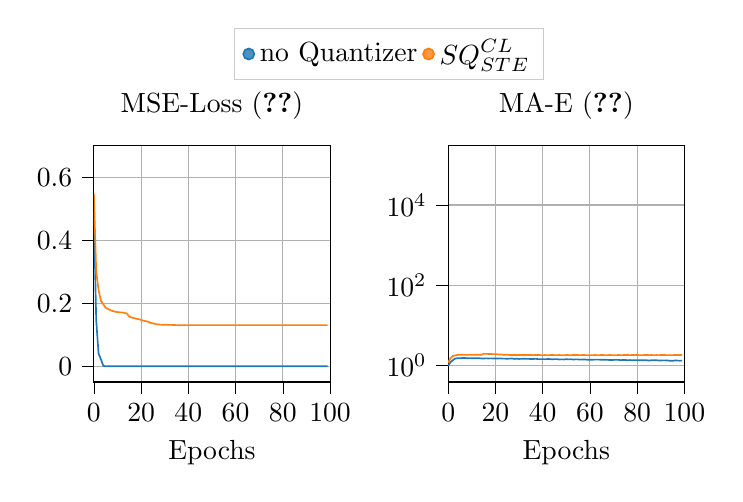
\begin{tikzpicture}

\definecolor{darkgray176}{RGB}{176,176,176}
\definecolor{darkorange25512714}{RGB}{255,127,14}
\definecolor{lightgray204}{RGB}{204,204,204}
\definecolor{steelblue31119180}{RGB}{31,119,180}

\begin{axis}[
name = plot1,
    width=3cm,  % Adjust the width of the plot
    height=3cm,  % Adjust the height of the plot
    scale only axis, 
    xlabel={Epochs},
legend cell align={center},
legend style={
  fill opacity=0.8,
  draw opacity=1,
  text opacity=1,
  at={(1.25,1.5)},
  anchor=north,
  draw=lightgray204,
  legend columns = -1
  mark=*
},
legend image code/.code={
        \draw[mark options={scale=1}, mark=*] plot coordinates {(0.3cm,0cm)}; % Use points in the legend
    },
tick align=outside,
tick pos=left,
x grid style={darkgray176},
xmajorgrids,
xmin=0, xmax=100,
xtick style={color=black},
y grid style={darkgray176},
ylabel={},
title={MSE-Loss (\ref{equ:MSELoss})},
ymajorgrids,
ymin=-0.05, 
ymax=0.7,
ytick style={color=black},
]
\addplot [semithick, steelblue31119180]
table {%
0 0.491439277626574
1 0.145839979875833
2 0.040147550188005
3 0.0221479450738989
4 0.00149579956594971
5 0.000185314791179735
6 2.88211019144455e-05
7 9.26099238910183e-06
8 5.63369642819112e-06
9 4.19628487658485e-06
10 3.45550454594701e-06
11 3.07767361245226e-06
12 2.69274032850575e-06
13 2.5199281473185e-06
14 2.32981874470539e-06
15 2.34445380689152e-06
16 2.23870044637131e-06
17 2.18607506899549e-06
18 2.14165844633563e-06
19 2.14033544194869e-06
20 2.19737296721045e-06
21 1.99292602428924e-06
22 2.05227904789707e-06
23 2.06425206110727e-06
24 2.0497238110101e-06
25 2.09024653652873e-06
26 1.96800227211469e-06
27 1.98377456345733e-06
28 2.04983100771627e-06
29 1.93138959105754e-06
30 1.97143960096093e-06
31 1.96656108060764e-06
32 1.96128012035343e-06
33 1.87406848142269e-06
34 1.95899548123064e-06
35 2.06950092014527e-06
36 1.77598596714649e-06
37 1.89258909054116e-06
38 1.86770988570095e-06
39 1.90023664551175e-06
40 1.98853274846311e-06
41 1.73420043834979e-06
42 1.83053138744999e-06
43 1.83887237433022e-06
44 1.84024018024732e-06
45 1.90997533066628e-06
46 1.73806030858443e-06
47 1.80118299307216e-06
48 1.77944000292866e-06
49 1.76767705089595e-06
50 1.78103714961068e-06
51 1.75996178718733e-06
52 1.79876262444878e-06
53 1.68875101220228e-06
54 1.72277751419593e-06
55 1.74380437144303e-06
56 1.65202610490772e-06
57 1.76343048156535e-06
58 1.62815765590901e-06
59 1.71006245526205e-06
60 1.67780812488743e-06
61 1.72043847649969e-06
62 1.65427349096531e-06
63 1.60840335319814e-06
64 1.6785292990398e-06
65 1.62734447482625e-06
66 1.66653455679233e-06
67 1.55285236923791e-06
68 1.59857226366006e-06
69 1.5729478062908e-06
70 1.58914339040814e-06
71 1.55204935845105e-06
72 1.56630324249829e-06
73 1.57998718153763e-06
74 1.52933544721759e-06
75 1.59393987128011e-06
76 1.61161236163954e-06
77 1.4681082392279e-06
78 1.52794630263894e-06
79 1.49592511971763e-06
80 1.48590521772443e-06
81 1.55174371780464e-06
82 1.41478302101003e-06
83 1.49139737778946e-06
84 1.48048299807561e-06
85 1.51897484758891e-06
86 1.38714931934843e-06
87 1.49776836886953e-06
88 1.41997981466642e-06
89 1.47431763927672e-06
90 1.42272246303093e-06
91 1.4149008913151e-06
92 1.39491322596242e-06
93 1.43892097185226e-06
94 1.3585801499705e-06
95 1.36681164034219e-06
96 1.38891166662127e-06
97 1.37259174018019e-06
98 1.36007890725973e-06
99 1.33940678363167e-06
};
\addlegendentry{no Quantizer}
\addplot [semithick, darkorange25512714]
table {%
0 0.549000259801745
1 0.299871038094163
2 0.242189251571894
3 0.207308624267578
4 0.197074625216424
5 0.185634178325534
6 0.182380964674056
7 0.178326630882919
8 0.175201226659119
9 0.173283803023398
10 0.172094418533146
11 0.171343371406198
12 0.170765378408134
13 0.169521951183677
14 0.167103111922741
15 0.157875367105007
16 0.154614733763039
17 0.153081586278975
18 0.150951494216919
19 0.149476350657642
20 0.147199265860021
21 0.144910294152796
22 0.143213532932103
23 0.14128946762532
24 0.137701354525983
25 0.136567906014621
26 0.134132204532623
27 0.132960757054389
28 0.132355139888823
29 0.131965770825744
30 0.131745044507086
31 0.131587471209466
32 0.13147689602524
33 0.131349040202796
34 0.131103035457432
35 0.130517799466848
36 0.130464115925133
37 0.130513427942991
38 0.130506151787937
39 0.130541185207665
40 0.130534353867173
41 0.130492865376174
42 0.130522380650043
43 0.130526529125869
44 0.130550112396479
45 0.130531256340444
46 0.130503811851144
47 0.130515778191388
48 0.130510073944926
49 0.130536538757384
50 0.130526625037193
51 0.130501929484308
52 0.130520934864879
53 0.130509537316859
54 0.130512963078916
55 0.130522072032094
56 0.130513535268605
57 0.130511100739241
58 0.130539780512452
59 0.130513597756624
60 0.130501266375184
61 0.130528594397008
62 0.130528959475458
63 0.130543941237032
64 0.130528621524572
65 0.130521844916046
66 0.130523137196898
67 0.130502953402698
68 0.130502688154578
69 0.130511386707425
70 0.130524727001786
71 0.130521879352629
72 0.130487557888031
73 0.130523864358664
74 0.130489279292524
75 0.130496246568859
76 0.130508339770138
77 0.130523177161813
78 0.130494157969952
79 0.130501418083906
80 0.130529735192657
81 0.130518131420016
82 0.130508684828877
83 0.130500476054847
84 0.130506072625518
85 0.130520362116396
86 0.13052210765332
87 0.130500621564686
88 0.130523995541036
89 0.130495601221919
90 0.130508861780167
91 0.130531919181347
92 0.130510828539729
93 0.130509101711214
94 0.130512753784657
95 0.130492839120328
96 0.130500469848514
97 0.130490967720747
98 0.130495262987912
99 0.130493671834469
};
\addlegendentry{$\text{SQ}^{\text{CL}}_\text{STE}$ }
\end{axis}



\begin{axis}[
        at={(plot1.east)}, % Align it next to the first plot
    anchor=west,
    width=3cm,  % Adjust the width of the plot
    height=3cm,  % Adjust 
     xshift=1.5cm, %the height of the plot
    scale only axis, 
    title={MA-E (\ref{equ:MAE})},
log basis y={10},
tick align=outside,
tick pos=left,
x grid style={darkgray176},
xlabel={Epochs},
xmajorgrids,
xmin=0, xmax=100,
xtick style={color=black},
y grid style={darkgray176},
ymajorgrids,
ymin=0.37772735089694, ymax=302220.574977491,
ymode=log,
ytick style={color=black}
]
\addplot [semithick, steelblue31119180]
table {%
0 0.967797929048538
1 1.18999158143997
2 1.3280640522639
3 1.45739589532216
4 1.48696814775467
5 1.49455015858014
6 1.4984413087368
7 1.50753791928291
8 1.48351823091507
9 1.49526984492938
10 1.48783353964488
11 1.47498019933701
12 1.48275196949641
13 1.48674787680308
14 1.46704434951146
15 1.4647004087766
16 1.47203040917714
17 1.46624130010605
18 1.47390285730362
19 1.46274871031443
20 1.45827481945356
21 1.4549953798453
22 1.47385632594426
23 1.45014885862668
24 1.4484273036321
25 1.44306247830391
26 1.45101089477539
27 1.46076002319654
28 1.4252666870753
29 1.44686559240023
30 1.42446284294128
31 1.43271813591321
32 1.44545921683311
33 1.43073971271515
34 1.43180764913559
35 1.4184127052625
36 1.42323799530665
37 1.43259494105975
38 1.41359353661537
39 1.40981947978338
40 1.40724654197693
41 1.406930210193
42 1.41545903881391
43 1.41366568605105
44 1.3914620300134
45 1.41088707844416
46 1.41070099075635
47 1.38227074742317
48 1.38994129101435
49 1.38415230512619
50 1.40318608283997
51 1.39011055628459
52 1.39560886224111
53 1.38020410339038
54 1.39084505240122
55 1.38685316840808
56 1.36806154648463
57 1.38207839330037
58 1.3816189746062
59 1.35772135059039
60 1.35888500610987
61 1.36058977842331
62 1.37051539222399
63 1.36771312554677
64 1.36801095207532
65 1.35492933392525
66 1.36689975063006
67 1.35233320991198
68 1.34628750681877
69 1.34210849801699
70 1.34686796466509
71 1.35329723159472
72 1.3503042280674
73 1.33104382157326
74 1.34038360118866
75 1.33892426292102
76 1.324663601319
77 1.33607966899872
78 1.32023986379306
79 1.31750364899635
80 1.32620007594426
81 1.31737558444341
82 1.31540066798528
83 1.32045937975248
84 1.32427805860837
85 1.29337703386943
86 1.32230117917061
87 1.32707501451174
88 1.32695627212524
89 1.30781185030937
90 1.30090575218201
91 1.31222044229507
92 1.3084713101387
93 1.3018348634243
94 1.2810719927152
95 1.27780377070109
96 1.30311262607574
97 1.29654068748156
98 1.288038311402
99 1.29606095949809
};
\addplot [semithick, darkorange25512714]
table {%
0 1.15177705486616
1 1.49898407856623
2 1.68984109958013
3 1.74100794792175
4 1.81043399969737
5 1.80887944698334
6 1.81068992614746
7 1.80273396571477
8 1.79722727139791
9 1.80120892524719
10 1.79876539707184
11 1.8107432325681
12 1.81065675814947
13 1.82434448401133
14 1.8075327595075
15 1.9066148519516
16 1.90987679560979
17 1.90051119724909
18 1.88925451437632
19 1.88267554442088
20 1.87240897019704
21 1.85495265722275
22 1.84392866690954
23 1.8233410914739
24 1.80795597235362
25 1.81095338265101
26 1.7882888674736
27 1.79436893860499
28 1.7830516854922
29 1.78319657246272
30 1.78521246512731
31 1.78399416208267
32 1.77897806962331
33 1.78484630187352
34 1.78965667883555
35 1.78724503119787
36 1.77722928126653
37 1.78671556711197
38 1.78292543490728
39 1.77811615069707
40 1.77549083630244
41 1.78069831530253
42 1.77355553309123
43 1.77956559658051
44 1.78367565870285
45 1.77791599432627
46 1.77011037667592
47 1.7834709127744
48 1.77421322266261
49 1.77529484033585
50 1.78160897095998
51 1.77904099623362
52 1.77556119362513
53 1.78328501383464
54 1.78391941785812
55 1.78135044972102
56 1.7737685362498
57 1.78358612060547
58 1.77882724603017
59 1.7719974120458
60 1.77522218624751
61 1.77480307420095
62 1.77991149822871
63 1.77920944690704
64 1.77348047494888
65 1.78633494377136
66 1.77663913567861
67 1.77468335231145
68 1.78009341160456
69 1.78007904291153
70 1.77263360420863
71 1.77128464778264
72 1.7840326944987
73 1.77595264911652
74 1.77936276594798
75 1.78149652481079
76 1.78397656679153
77 1.77532234191895
78 1.78522520860036
79 1.77818075418472
80 1.78747274080912
81 1.77702915668488
82 1.77857061624527
83 1.77995453675588
84 1.7965615272522
85 1.77666591008504
86 1.78238356908162
87 1.77309301694234
88 1.78007437785467
89 1.77789382537206
90 1.78000446160634
91 1.78402543465296
92 1.78007783095042
93 1.77365928490957
94 1.78022813002268
95 1.77402989466985
96 1.78552823464076
97 1.77882620096207
98 1.78523919582367
99 1.7766180674235
};
\end{axis}
\end{tikzpicture}
